\documentclass {article}
\usepackage{fullpage}
\usepackage{parskip}
\usepackage{minted}
\usepackage{float}
\usepackage{graphicx}
\usepackage{hyperref}
\hypersetup{
    colorlinks=false,
    linkcolor=blue,
    filecolor=magenta,
    urlcolor=cyan,
}

% biblatex setup
\usepackage[style=numeric,backend=biber,sorting=none]{biblatex} % use biber and order references as they appear
\addbibresource{references.bib} % biblatex file
\emergencystretch=1em % prevent overflow of bib

\DeclareUnicodeCharacter{2500}{-}
\DeclareUnicodeCharacter{251C}{|}
\DeclareUnicodeCharacter{2502}{|}
\DeclareUnicodeCharacter{2514}{|}


\begin{document}

~\vfill
\begin{center}
\Large

CS488 Project Documentation

Title: Kefka --- First-Person Shooter Game Engine

Name: Zac Joffe

Student ID: 20711812

User ID: zmjoffe

\end{center}
\vfill ~\vfill~

\newpage
\tableofcontents

\newpage
\section{Project Outline}
\subsection{Purpose}
To create a 3D environment that can be explored via a first-person perspective.

\subsection{Background \& Motivation}\label{sec:background}
I've always been interested in creating a 3D game engine using OpenGL. First-person shooters have been one of my favourite game genres for well over a decade \footnote{Standout titles of the genre include \textit{Doom}, \textit{Quake}, \textit{Blood}, \textit{Half-Life}, \textit{Portal 2}, and \textit{Metroid Prime}.}. This project is primarily focused on the graphics engine; the gameplay is simple and serves as an interesting context for the implementation of the graphics component. The player controls a character equipped with a firearm in a first-person point of view. The gun can be used to shoot enemies that move in the environment. The player can freely move about the world on the ground-level and look around the environment, just as one would expect from a first-person shooter.

This project was challenging since it employed a wide range of graphics concepts. Nearly all concepts in the pre-ray tracing part of the course were employed, and implementation of each objective was non-trivial. Through this project, I learned how to create a basic 3D game engine which can be used to create a simple first-person shooter. Moreover, I learned a lot about how to architect a game engine. Large parts of the codebase were refactored throughout the development process in order to facilitate new functionality and improve component flexibility. Since much of the ``how'' of implementation was researched during development \footnote{The high-level research I did for the proposal was certainly helpful in implementing the objectives. The ``how'' here refers to the lower level implementation details.}, I made many poor decisions that resulted in a lot of extra work. I believe that is part of the learning process with a project of this scale, and is most certainly expected with my level of experience using OpenGL. Section~\ref{sec:implementation} documents implementation details of the final code revision.

\subsubsection{What is a ``Kefka''?}
The name ``Kefka'' comes from the main antagonist of my favorite game, \href{https://en.wikipedia.org/wiki/Final_Fantasy_VI}{\textit{Final Fantasy VI}}. I've thought of this project as the ``final boss'' of my degree, so this name felt appropriate.

\section{Development}
\subsection{Development Environment}\label{sec:devenv}
The project was primarily developed on my desktop with an AMD 5950x and an Nvidia RTX 3090 running Arch Linux with the latest stable kernel. I briefly tested it on my Framework Laptop with an Intel Core i5 240p (integrated graphics), also running Arch Linux with the latest stable kernel. I also made sure it compiled on the CS488 virtual machine before submission.

Git was used as my version control system. I made an attempt to make each commit represent a feature/bugfix/change so I could leverage \texttt{git bisect} if needed.

The project source is written in C++17, and I (naturally) used Emacs to write all code. The only reason I mention the latter is that my submitted directory includes files \texttt{.projectile} and \texttt{.dir-locals.el}, which are used to help configure my Emacs environment. These can be safely ignored.

\subsection{Project Metadata}
It goes without saying that this project was a lot of work. This subsection is a fun, albeit brief, analysis of the amount of work I put in.

A good place to begin is by showing the number of commits to the master branch:
\begin{minted}[fontsize=\small]{sh}
zac@arch ~/D/C/cs488-project (master) [SIGHUP]> git rev-list --count master
144
\end{minted}

As mentioned in section~\ref{sec:devenv}, most commits contain a single feature/bugfix/change, so the size of each commit varies widely. Using \texttt{git log} and some shell-fu we can see how many lines of code were inserted and deleted over the 144 commits. Note that this is only files in the \texttt{src} directory, as this is where all the C++ source/header files I wrote live. Many more lines were written outside this directory in the form of vertex/fragment shaders, build scripts, and modifications to the CS488 framework.
\begin{minted}[fontsize=\small]{sh}
zac@arch ~/D/C/cs488-project (master)> git log --author="Zac Joffe" --pretty=tformat: --numstat -- src/ \
  | awk '{ inserted+=$1; deleted+=$2 } END { print "Lines inserted: " inserted, "Lines deleted: " deleted }'
Lines inserted: 5395 Lines deleted: 2826
\end{minted}

I wrote a lot of code! And deleted a lot of it too. As mentioned in section~\ref{sec:background}, I had to refactor and rearchitect quite often throughout development, which explains the numbers above.

Using the \href{https://github.com/boyter/scc}{\texttt{scc}} tool, we can see some interesting metadata about the C++ source/header files in the \texttt{src} directory:
\begin{minted}[fontsize=\small]{sh}
zac@arch ~/D/C/c/src (master)> scc .
───────────────────────────────────────────────────────────────────────────────
Language                 Files     Lines   Blanks  Comments     Code Complexity
───────────────────────────────────────────────────────────────────────────────
C Header                    20       894      200        17      677          0
C++                         18      1675      318        78     1279        145
Emacs Lisp                   1         1        0         0        1          0
───────────────────────────────────────────────────────────────────────────────
Total                       39      2570      518        95     1957        145
───────────────────────────────────────────────────────────────────────────────
Estimated Cost to Develop (organic) \$54,672
Estimated Schedule Effort (organic) 4.56 months
Estimated People Required (organic) 1.07
───────────────────────────────────────────────────────────────────────────────
Processed 73866 bytes, 0.074 megabytes (SI)
───────────────────────────────────────────────────────────────────────────────
\end{minted}
I'm not quite sure how the ``Cost to Develop'' metric is measured, though I must say it's a humbling number!

\section{Manual}\label{sec:manual}
\subsection{Building \& Running}
The submitted \texttt{cs488-project.zip} file includes the \texttt{cs488-project} directory, which has a similar structure to the \texttt{cs488} starter code provided for assignments at the start of the term. The \texttt{cs488-project} directory will be referred to as the ``root'' or ``project root'' directory. \texttt A detailed explanation of the project structure can be found in section~\ref{sec:structure}. The build system was simplified to use a single \texttt{premake4} build script.

To build the code, run the \texttt{premake4} script from the root directory as follows:
\begin{minted}[fontsize=\small]{sh}
$ premake4 gmake && make
\end{minted}

This will compile and link all the necessary libraries and project files. The resulting binary, \texttt{fps}, is outputted in the current working directory. All libraries are statically linked, but the asset paths are dynamically loaded at runtime. Therefore, the binary must be ran with the project root the current working directory. Running the binary is done as follows:
\begin{minted}[fontsize=\small]{sh}
$ ./fps
\end{minted}

There are no command line arguments (or, rather, any provided arguments will be ignored). The game will launch in a window with a resolution of \texttt{1024 x 768}, and is not designed to be resized \footnote{Resizing the window in the main menu before starting the game will make the game render correctly at the new resolution. Resizing the window when playing the game will cause distortions.}. The name of the window is \texttt{CS488\_Project\_FPS}.

\subsection{Main Menu}
When the game starts, the player is presented with the main menu, which is shown in figure~\ref{fig:mainmenu}.

\begin{figure}[H]
  \begin{center}
  \includegraphics[width=\textwidth]{main\_menu.png}
  \end{center}
  \caption{Screenshot of main menu}\label{fig:mainmenu}
\end{figure}

The main menu contains two buttons: ``Start Game'' and ``Options''. The ``Start Game'' button, as one might expect, exits the main menu and starts the game. The ``Options'' button opens a submenu containing a number of widgets to customize the game experience. A screenshot of the options submenu is shown in figure~\ref{fig:optionsmenu}.
\begin{figure}[H]
  \begin{center}
  \includegraphics[width=\textwidth]{options\_menu.png}
  \end{center}
  \caption{Screenshot of options submenu with default game parameters}\label{fig:optionsmenu}
\end{figure}

The ``World Size'' slider tweaks the size of the $N \times N$ world of the game on the horizontal ($xz$) plane. See section~\ref{sec:modelscene} for more details about game world. This slider lets you pick integers in the range of $[20, 75]$.

The ``Num Enemies'' slider tweaks the number of enemies that spawn in the world. This slider lets you pick integers in the range of $[3, 10]$.

The ``Floor Texture'' list box selects the texture that is used to map onto the floor of the game world. Similarly, the ``Wall Texture'' and ``Enemy Texture''\footnote{The ``Mayahem'' family of textures are different stones. The name is a reference to the first level in \href{https://en.wikipedia.org/wiki/Banjo-Tooie}{\textit{Banjo-Tooie}}, \textit{Mayahem Temple}, where the titular hero Banjo transforms into a \href{https://banjokazooie.fandom.com/wiki/Stony_Banjo}{``Stony''} to play in a kickball tournament.} list boxes select the texture used to map onto the walls and enemies in the world, respectively. The ``Skybox'' list box selects the set of textures used to form the skybox.

The ``Back to Main Menu'' button goes back to the parent main menu. Note that parameters are automatically saved after being tweaked, so starting the game from the main menu will start it with the parameters outlined in the options submenu.

At any point in any menu, the \texttt{escape} key can be pressed to close the window. Additionally, the \texttt{s} key will start the game in either menu.

\subsection{The Game}\label{sec:game}
The game consists of an $N \times N$ world that the player spawns in. Players are free to move within the $N \times N$ world, though they cannot move outside of the world boundaries defined by the walls. Enemies move spawn in random locations and move around the world randomly. If a player shoots an enemy, they will fall to the ground and stop moving. Note that there are no strict objectives to the game, and thus no win or lose states. A screenshot of the game is shown in figure~\ref{fig:game}.
\begin{figure}[H]
  \begin{center}
  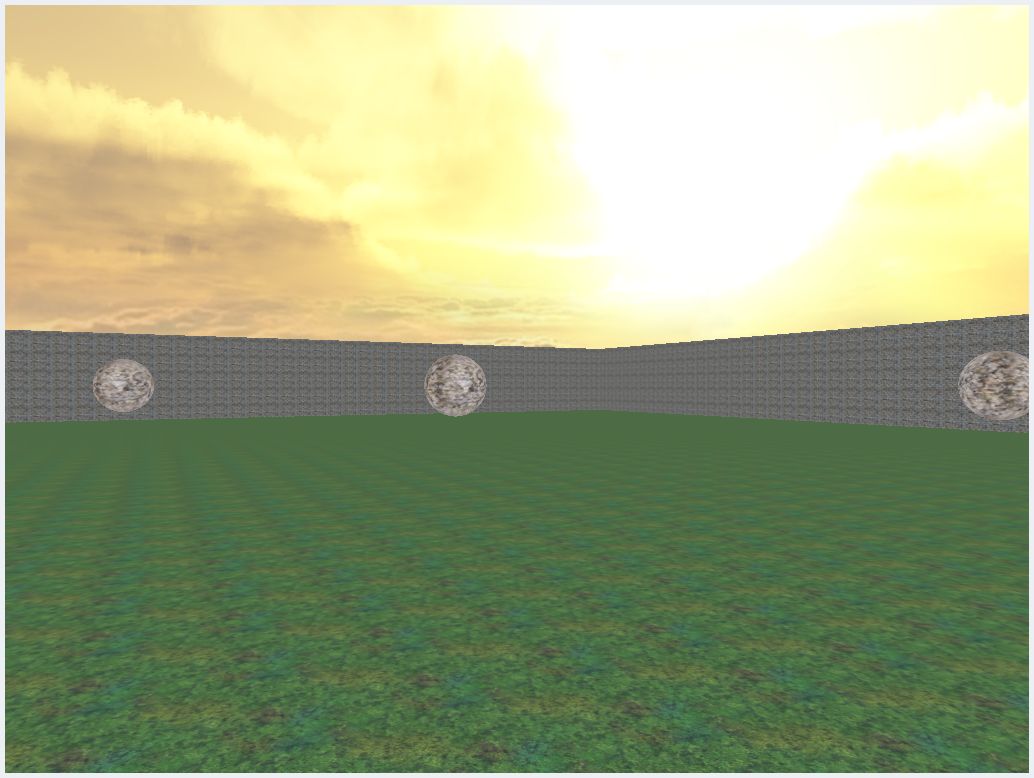
\includegraphics[width=\textwidth]{game.png}
  \end{center}\caption{Screenshot of game with default game parameters}\label{fig:game}
\end{figure}

\subsubsection{Game Controls}\label{sec:controls}
The game is controlled using the mouse and keyboard. If you've played a first-person shooter in the last 25 years, the controls should feel familiar and intuitive. An outline of the game controls is as follows:
\begin{itemize}
  \item \texttt{w}: Move forward.
  \item \texttt{a}: Move (strafe) left.
  \item \texttt{s}: Move back.
  \item \texttt{d}: Move (strafe) right.
  \item \texttt{space}: Jump.
  \item \texttt{left shift}: Hold to sprint (increase movement speed cap).
  \item \texttt{r}: Respawn all enemies.
  \item \texttt{escape}: Close the window.
  \item \texttt{left mouse button}: Shoot gun.
\end{itemize}

The mouse is used to look around the world. That is, moving the mouse in a direction moves rotates the camera in that direction accordingly.

\section{Implementation}\label{sec:implementation}
C++17 was used to write the project. I made an attempt to use modern C++ techniques, which is hopefully evident throughout much of the source code.

\subsection{Project Structure}\label{sec:structure}
The project layout is based on the CS488 assignment folder. The output of \texttt{tree -L 2 -d} in the root directory shows the directory structure:
\begin{minted}[fontsize=\small]{sh}
.
├── assets
│   ├── fonts
│   ├── meshes
│   ├── shaders
│   ├── sounds
│   └── textures
├── lib
├── shared
│   ├── cs488-framework
│   ├── gl3w
│   ├── glfw-3.3
│   ├── imgui
│   ├── include
│   ├── lua-5.3.1
│   └── soloud
└── src
\end{minted}

The \texttt{assets} directory contains all the relevant assets that that are dynamically loaded at runtime. Note that the \texttt{assets/shaders} directory contains vertex/fragment shaders written in GLSL. The \texttt{lib} directory contains statically built libraries. The \texttt{shared} directory contains the source and headers of the libraries used in the project. The C++ source and header files live inside the \texttt{src} directory.

Note that other directories and files may be generated by the build scripts.

\subsubsection{Modifications to CS488 Framework}
The build process for normal CS488 assignments involve building the static libraries in the root directory, then compiling and linking assignment code in their respective directories. I've simplified this process to use a single \texttt{premake4} script, which builds all static libraries, and compiles and links the project source code.

I've updated ImGui to the latest release (which at the time of writing is \href{https://github.com/ocornut/imgui/releases/tag/v1.89.4}{v1.89.4}). The version of ImGui packaged with the CS488 starter code seemed to be around 8 years old, and updating it gave me access to the modern ImGui interfaces that are referred to in the documentation. The update required modifying the CS488 framework code to leverage updated ImGui functions.

I wrote a composition-based wrapper of the \texttt{ShaderProgram} class from the CS488 framework. The class definition for this wrapper is as follows:
\begin{minted}[fontsize=\small]{C++}
class ShaderHandler {
public:
    ShaderHandler(const std::string & vertex_filename, const std::string & fragment_filename);
    ~ShaderHandler();

    void enable();
    void disable();

    void uploadMat4Uniform(const std::string & name, const glm::mat4 & m) const;
    void uploadVec2Uniform(const std::string & name, const glm::vec2 & v) const;
    void uploadVec3Uniform(const std::string & name, const glm::vec3 & v) const;
    void uploadVec4Uniform(const std::string & name, const glm::vec4 & v) const;

private:
    ShaderProgram m_shader;
};
\end{minted}

This class further cleans up shader management, which is especially helpful since the project uses 3 sets of shaders.

\subsection{Objective 1: Modeling the Scene}\label{sec:modelscene}
The scene consists of four sets of objects:
\begin{enumerate}
  \item Skybox
  \item Floors
  \item Walls
  \item Enemies
\end{enumerate}

These objects are encapsulated into a \texttt{Scene} class, which is defined as follows:
\begin{minted}[fontsize=\small]{C++}
class Scene {
public:
    Scene(const GameContext & game_context);

    void draw(const glm::mat4 & projection, const glm::mat4 & view, const glm::mat4 & model) const;
    std::list<BoundingBox> getStaticCollidableObjects() const;
    std::list<BoundingBox> getAllCollidableObjects() const;
    void handleShot(const Ray & ray);
    void tick(float delta_time);
    void respawnEnemies();

private:
    ... // elided for brevity
    std::shared_ptr<ShaderHandler> m_shader_handler;
    std::shared_ptr<Texture> m_floor_texture;
    Tiles m_floor;

    std::shared_ptr<Texture> m_wall_texture;
    std::array<Tiles, 4> m_walls;

    std::shared_ptr<Texture> m_enemy_texture;
    std::list<Enemy> m_enemies;

    std::shared_ptr<ShaderHandler> m_skybox_shader_handler;
    std::unique_ptr<Skybox> m_skybox;
    ... // elided for brevity
};
\end{minted}

The \texttt{Tile} class models a single 2D square tile defined on the $xz$ plane with side lengths and an area of 1. The vertices are defined as follows:
\begin{minted}[fontsize=\small]{C++}
static const float VERTICES[NUM_VERTICES * 3] = {
    // x    y    z
    0.0f, 0.0f, 1.0f,  // front left
    0.0f, 0.0f, 0.0f,  // back left
    1.0f, 0.0f, 0.0f,  // back right
    1.0f, 0.0f, 1.0f   // front right
};

static const GLuint NUM_INDEXES = 6;
static const GLuint VERTICES_INDEXES[NUM_INDEXES] = {
    0, 1, 2,
    2, 3, 0,
};
\end{minted}

The \texttt{VERTICES\_INDEXES} is used for an element buffer object to clean up the vertex definition. The \texttt{Tile::draw} draws the instance of the tile.

The \texttt{Tiles} class wraps a vector of \texttt{Tile}s, which is useful for when we need to store a dynamic number of tiles. In particular, the number of tiles in the floor and each wall is defined by the size of the world, which is parameterized in the game context. It comes naturally from this that the floor is stored as an instance of \texttt{Tiles} and the walls as a fixed array of 4 \texttt{Tiles}.

Enemies are defined as spherical meshes, which were created in Blender. The mesh is dynamically loaded using the \texttt{ObjFileDecoder::decode} method in a similar fashion to how it was done in assignments 3 and 4. The \texttt{Enemy} class encapsulates all the buffers related to the instance of the enemy, and the \texttt{Enemy::draw} method draws the enemy in the world.

The \texttt{Skybox} class uses vertices of a cube map to form the skybox, and is drawn with the \texttt{Skybox::draw} method. It's worth noting that the skybox has its own vertex/fragment shader, which strips the translation part of the view matrix so that the skybox appears to stay stationary when the player moves around the world.

The \texttt{Scene::draw} method is responsible for drawing all renderable objects. The code for the method is as follows:
\begin{minted}[fontsize=\small]{C++}
void Scene::draw(const glm::mat4 & projection, const glm::mat4 & view, const glm::mat4 & model) const {
    m_skybox->draw(projection, view);

    m_shader_handler->enable();
    m_shader_handler->uploadMat4Uniform("projection", projection);
    m_shader_handler->uploadMat4Uniform("view", view);
    m_shader_handler->uploadMat4Uniform("model", model);

    glActiveTexture(GL_TEXTURE0);
    m_floor.draw();

    for (const auto & wall : m_walls) {
        glActiveTexture(GL_TEXTURE1);
        wall.draw();
    }

    for (const auto & enemy : m_enemies) {
        glActiveTexture(GL_TEXTURE1);
        enemy.draw(projection, view);
    }

    m_shader_handler->disable();
    glBindVertexArray(0);
}
\end{minted}

This method is responsible for drawing all the objects that are stored in the scene and is called every frame during gameplay.

\subsection{Objective 2: UI}\label{sec:ui}
In order to make a main menu, we need to a way to render a completely different scene with a completely different state. That's where the state pattern comes into play~\cite{gofstate}~\cite{gamestate}. For this pattern, the pure virtual struct \texttt{State} defines a common interface that that \texttt{Window} can use to run app logic, GUI logic, and drawing:
\begin{minted}[fontsize=\small]{C++}
struct State {
    virtual ~State() {}

    virtual void appLogic(float delta_time) = 0;
    virtual void guiLogic(const std::unique_ptr<GameContext> & game_context) = 0;
    virtual void draw() = 0;
    virtual void handleMouseMove(double xpos, double ypos) = 0;
    virtual void handleMouseButtonInput(int button, int actions, int mods) = 0;
    virtual bool handleKeyInput(int key, int action, int mods) = 0; // returns true if window should close
    virtual bool switchStates() = 0;
};
\end{minted}

A unique pointer to \texttt{State} is stored as a member in \texttt{Window}. Note that the \texttt{Window} class is largely the same as the ones from assignments 1, 2, and 3. As \texttt{State} is pure virtual, this member must point to a concrete implementation of the interface, of which there are 2: \texttt{MenuState} and \texttt{GameState}. The \texttt{MenuState} class implements all the logic for the main menu, and the \texttt{GameState} class contains the scene, camera, and everything else that is needed for the actual game. Comparing this to the assignments again, the \texttt{GameState} class abstracts a lot of the state that was (presumably) stored in \texttt{Window}.

The \texttt{MenuState} implementation leverages ImGui for the UI, where the menus are defined in \texttt{MenuState::guiLogic}. When the ``Start Game'' button is pressed, \texttt{Window} switches its state pointer to a new instance of \texttt{GameState}.

The \texttt{GameContext} struct defines the game parameters that can be tweaked from the options submenu:
\begin{minted}[fontsize=\small]{C++}
struct GameContext {
    unsigned int num_enemies;
    unsigned int world_size;
    int floor_texture;
    int wall_texture;
    int enemy_texture;
    int skybox;
    GameContext() :
        num_enemies(game_context_constants::DEFAULT_NUM_ENEMIES),
        world_size(game_context_constants::DEFAULT_WORLD_SIZE),
        floor_texture(0),
        wall_texture(0),
        enemy_texture(0),
        skybox(0) {}
};
\end{minted}

A unique pointer to an instance of \texttt{GameContext} is stored as a member in \texttt{Window}. This instance is passed to the \texttt{State::guiLogic} method and is modified when interacting with the options submenu. When changing state, this instance is injected into the \texttt{GameState} constructor and is used to adjust the game accordingly.

\subsection{Objective 3: Texture Mapping}
The approach to implementing texture mapping in OpenGL largely the same as that first described by Blinn and Newell~\cite{texture}. 2D texture rasters are loaded from the \texttt{assets/textures} into memory using the stb image loader library. The texture is then uploaded to the GPU from memory through calls to the OpenGL API. The texture coordinates of a mesh ($u, v$) are passed as input to the vertex shader, which outputs it to the fragment shader. The fragment shader uses the input texture coordinates to determine the fragment's color.


This business logic behind texture loading/initialization is encapsulated in the \texttt{Texture} class, which is defined as follows:
\begin{minted}[fontsize=\small]{C++}
class Texture {
public:
    Texture(const std::string & filename);

    void bind(GLenum texture_unit) const;

private:
    std::string m_filename;
    GLuint m_tex;
};
\end{minted}

The constructor loads the texture from disk and creates all the necessary buffers on the GPU. The following code sets the texture filtering options which make OpenGL perform bilinear interpolation of the texels surrounding texture coordinates to calculate the color. It also generates the mipmaps and enables mipmapping.
\begin{minted}[fontsize=\small]{C++}
glTexParameteri(GL_TEXTURE_2D, GL_TEXTURE_WRAP_S, GL_REPEAT);
glTexParameteri(GL_TEXTURE_2D, GL_TEXTURE_WRAP_T, GL_REPEAT);
glTexParameteri(GL_TEXTURE_2D, GL_TEXTURE_MIN_FILTER, GL_LINEAR_MIPMAP_LINEAR);
glTexParameteri(GL_TEXTURE_2D, GL_TEXTURE_MAG_FILTER, GL_LINEAR);

// load image from disk into data, image width into x, image height into y (omitted)

glTexImage2D(GL_TEXTURE_2D, 0, GL_RGBA, x, y, 0, GL_RGBA, GL_UNSIGNED_BYTE, data);

glGenerateMipmap(GL_TEXTURE_2D);
\end{minted}

Calls to the \texttt{Texture::bind} method bind the texture associated with the \texttt{Texture} instance to subsequently drawn meshes.

The texture coordinates for the spherical mesh are generated by Blender and hardcoded into its \texttt{.obj} file. The texture coordinates for \texttt{Tile}s are defined statically in code as follows:
\begin{minted}[fontsize=\small]{C++}
static const float UV_COORDS[NUM_VERTICES * 2] = {
    0.0f, 0.0f,  // front left
    0.0f, 1.0f,  // back left
    1.0f, 1.0f,  // back right
    1.0f, 0.0f   // front right
};
\end{minted}

These are passed to the vertex shader in the same way as the texture coordinates for dynamically loaded meshes.

\subsection{Objective 4: Particle System}\label{sec:particles}
The particle system is used for displaying blood particles after shooting an enemy. The implementation of particle systems is modelled off a 2D implementation outlined in the \texttt{Particles} section of \textit{Learn OpenGL: Learn Modern OpenGL Graphics Programming in a Step-by-step Fashion.}~\cite{learnopengl}.

A particle is defined to be a small object --- in this case a cube mesh defined by \texttt{assets/meshes/cube.obj} --- that has a position, direction of movement, speed, and color. Note that particles are textured red and the color variance is based on the \texttt{color} field. Particles also have a life (time-to-death) that dictates how many ticks it is away from being killed, and a life counter that outlines how many lives the instance of the particle has been through. With that, here's the \texttt{Particle} struct definition:
\begin{minted}[fontsize=\small]{C++}
struct Particle {
    glm::vec3 pos;
    glm::vec3 velocity;
    glm::vec4 color;
    float life;
    unsigned int times_lived;
    Particle() : pos(0.0f), velocity(0.0f), color(1.0f), life(0.0f), times_lived(0) {}
};
\end{minted}

\texttt{Particle}s are used by the \texttt{ParticleEmitter} class, which is defined as follows:
\begin{minted}[fontsize=\small]{C++}
class ParticleEmitter {
public:
    ParticleEmitter(unsigned int num_particles);

    void emit(const glm::vec3 & position);
    void draw(const glm::mat4 & projection, const glm::mat4 & view) const;
    void tick(float delta_time,
              const glm::vec3 & position,
              unsigned int new_particles);

private:
    void initBuffers();
    void initParticle(Particle & particle, const glm::vec3 & position);
    size_t findFirstDeadParticle() const;

    // OpenGL buffer ids (omitted)

    std::vector<Particle> m_particles;

    // particle mesh data (omitted)

    // shader handler, texture, and other misc fields (omitted)

    unsigned int m_num_particles;

    Rng m_rng;
};
\end{minted}

The \texttt{ParticleEmitter::emit} method initializes particles with a random life, color, and velocity. It also places the particle in a random location around a defined circle, which gives the illusion that the particles are generated from the enemy. Particles that are killed are respawned if they have lived less than a set number of lives, as defined by the constant \texttt{DEFAULT\_MAX\_LIVES}. This constant is set to a value of 5.

Each frame, the delta time is calculated by the \texttt{Window::calculateDeltaTime} method:
\begin{minted}[fontsize=\small]{C++}
void Window::calculateDeltaTime() {
    const float current_frame_time = glfwGetTime();
    m_delta_time = current_frame_time - m_last_frame_time;
    m_last_frame_time = current_frame_time;
}
\end{minted}

Each \texttt{Enemy} stores its own instance of \texttt{ParticleEmitter}. Upon being shot, the enemy's blood particles are generated by calling the \texttt{ParticleEmitter::emit} method on its particle emitter. Every frame, particle emitters receive the delta time and use it to decrease the life of every alive particle. With the initial time-to-death being randomized, the particles spawn and die at a rate that creates the illusion of particles being continuously generated until they all die rather than being continuously spawned and killed. The reuse of existing particles with the life counter is an effective memory and performance optimization. Additionally, the \texttt{m\_particles} vector is cleared after all particles have died on their last life. Thus, time will not be spent each frame iterating through large vectors of dead particles.

\subsection{Objective 5: Synchronized Sound}
The \href{https://solhsa.com/soloud/}{\texttt{SoLoud}} high-level C++ audio library was used to implement sound. Most of the work consisted of modifying the build script to correctly build the library. Client code uses the library by interacting with the SoLoud engine core, making it a prime candidate for the singleton pattern. The singleton pattern, as first described by the Gang of Four in 1994~\cite{gofsingleton}, forces at most a single instance of a class to exist at runtime.

This \texttt{SoundEngine} class wraps the calls to the SoLoud API that we require to play sound files:
\begin{minted}[fontsize=\small]{C++}
class SoundEngine {
public:
    static SoundEngine & getInstance();
    SoundEngine(SoundEngine const &) = delete;
    void operator=(SoundEngine const &) = delete;

    void play(SoLoud::Wav & wav);
    void playIfAvailable(SoLoud::Wav & wav);

private:
    SoundEngine();

    SoLoud::Soloud m_soloud_engine;
};
\end{minted}

The singleton property is forced by deleting the copy assignment operator and copy constructor, and making the default constructor private. Client code wishing to use a \texttt{SoundEngine} must get an instance of it through the static \texttt{getInstance} method.

The sound files used are all dynamically loaded on initialization and stored in objects of type \texttt{SoLoud::Wav}. The \texttt{SoundEngine::play} method plays a loaded sound file once to completion. The \texttt{SoundEngine::playIfAvailable} method plays a loaded sound file if nothing else is playing. This is used to play footstep sounds without having them overlap.

Here are all the sounds that can play during gameplay:
\begin{itemize}
  \item Footstep: Plays when the player moves around the world on the ground level. Stops playing when the player is in midair after jumping.
  \item Jumping grunt: Plays when the player initiates a jump. Note that there are two grunting sounds which are randomly selected before playing.
  \item Gunshot: Plays when player shoots their gun.
\end{itemize}

\subsection{Objective 6: Static Collision Detection}\label{sec:static}
Static collision detection was implemented to prevent the player from moving out of the bounds defined by scene. That is, players are blocked by the walls surrounding the world and are unable to move passed them.

The player's location is surrounded by an invisible axis-aligned bounding box (AABB). This bounding box is implemented as a square living on the $xz$ plane. It is sufficient to store a pair of \texttt{glm::vec2} coordinates, with the first vector representing the minimum $x$ and $z$ values of the bounding box and the second vector representing the maximum $x$ and $z$ values of the bounding box. The \texttt{BoundingBox} struct is defined as follows:
\begin{minted}[fontsize=\small]{C++}
using LineSegment = std::pair<glm::vec2, glm::vec2>;

struct BoundingBox {
    glm::vec2 min;
    glm::vec2 max;
    BoundingBox();
    BoundingBox(glm::vec2 min, glm::vec2 max);

    bool collisionTest(const BoundingBox & other) const;
    std::string toString() const;

    std::list<LineSegment> getLineSegments() const;
};
\end{minted}

Most of the code is self explanatory. The \texttt{BoundingBox::getLineSegments} method is used for dynamic collision detection and is detailed in section~\ref{sec:dynamic}. The \texttt{BoundingBox::collisionTest} method calculates if the instance of \texttt{BoundingBox} collides with another \texttt{BoundingBox}:
\begin{minted}[fontsize=\small]{C++}
bool BoundingBox::collisionTest(const BoundingBox & other) const {
    return max.x >= other.min.x && other.max.x >= min.x
        && max.y >= other.min.y && other.max.y >= min.y;
}
\end{minted}

The \texttt{Camera} class stores the player's position and handles player movement with static collision testing. An instance of \texttt{BoundingBox} is stored in \texttt{GameState}. Each time the player moves, the bounding box is calculated with the following method:
\begin{minted}[fontsize=\small]{C++}
BoundingBox Camera::updateBoundingBoxHelper(const glm::vec3 & pos) const {
    return BoundingBox(
        glm::vec2(pos.x - BOUNDING_BOX_OFFSET, pos.z - BOUNDING_BOX_OFFSET),
        glm::vec2(pos.x + BOUNDING_BOX_OFFSET, pos.z + BOUNDING_BOX_OFFSET)
    );
}
\end{minted}
This is defined as a helper since the \texttt{Camera::move} method --- which is called every frame by \texttt{GameState::appLogic} --- uses this to calculate if a player's movement that frame results in a collision. The walls defined in \texttt{Scene} have instances of \texttt{BoundingBox} that don't change after initialization and are stored in their respective instances of \texttt{Tiles}. The \texttt{Scene::getStaticCollidableObjects} method returns a list of these wall \texttt{BoundingBox}es. The \texttt{Camera::updatePosition} method uses this list with the bounding box with the updated player position to test if said movement results in a collision:
\begin{minted}[fontsize=\small]{C++}
void Camera::updatePosition(const glm::vec3 & velocity, std::list<BoundingBox> collidable_objects) {
    const glm::vec3 new_pos = m_pos + velocity;
    const BoundingBox new_bounding_box = updateBoundingBoxHelper(new_pos);

    for (const auto & obj : collidable_objects) {
        if (new_bounding_box.collisionTest(obj)) {
            return;
        }
    }

    m_pos = new_pos;
    m_bounding_box_xz = new_bounding_box;
}
\end{minted}

Each enemy stores their own bounding box and updates it each frame in a similar manner to how it is done for the player. That is, a helper method, \texttt{Enemy::updateBoundingBoxHelper}, is ran each frame:
\begin{minted}[fontsize=\small]{C++}
BoundingBox Enemy::updateBoundingBoxHelper(const glm::vec3 & pos) const {
    return BoundingBox(
        glm::vec2(pos.x - BOUNDING_BOX_OFFSET, pos.z - BOUNDING_BOX_OFFSET),
        glm::vec2(pos.x + BOUNDING_BOX_OFFSET, pos.z + BOUNDING_BOX_OFFSET)
    );
}
\end{minted}

And, similar to player movement logic, collision with the surrounding walls is tested to prevent enemies from leaving the defined world:
\begin{minted}[fontsize=\small]{C++}
bool Enemy::tryUpdatePosition(const glm::vec3 & velocity, std::list<BoundingBox> collidable_objects) {
    const glm::vec3 new_pos = m_pos + velocity;
    const BoundingBox new_bounding_box = updateBoundingBoxHelper(new_pos);

    for (const auto & obj : collidable_objects) {
        if (new_bounding_box.collisionTest(obj)) {
            return false;
        }
    }

    m_pos = new_pos;
    m_bounding_box_xz = new_bounding_box;
    return true;
}
\end{minted}

The major difference between \texttt{Enemy::tryUpdatePosition} and \texttt{Camera::updatePosition} is that \\\texttt{Enemy::tryUpdatePosition} returns a \texttt{bool} to indicate if there was a collision. We don't want enemies to stop moving after getting stuck, so a simple \texttt{while} loop is used in conjunction with \texttt{Enemy::tryUpdatePosition} to find a random direction that does not result in a collision:
\begin{minted}[fontsize=\small]{C++}
while (!tryUpdatePosition(speed * m_move_direction, collidable_objects)) {
    m_move_direction = getRandomDirection();
}
\end{minted}

\subsection{Objective 7: Dynamic Collision Detection}\label{sec:dynamic}
As mentioned in the previous subsection, enemies move around the scene randomly. A dynamic collision detection algorithm is used to determine if a player's shot hits an enemy. This algorithm is called hitscanning, and is very similar to the ray casting algorithm as described in the ray tracing chapter of \textit{Fundamentals of Computer Graphics}~\cite{rtbook}.

When the player shoots their gun, a ray is be casted from the player/camera position the direction that the camera is facing. The \texttt{Ray} class is defined as follows:
\begin{minted}[fontsize=\small]{C++}
class Ray {
public:
    glm::vec3 e; // start position
    glm::vec3 d; // direction of ray

    Ray(glm::vec3 e, glm::vec3 d);
    glm::vec3 operator()(float t) const;
    bool collisionTestXZ(const std::list<LineSegment> & line_segments) const;

private:
    bool collisionTestHelper(const LineSegment & line_segment) const;
};
\end{minted}

Note that even though \texttt{Ray} is defined as a 3D vector, we only consider collision detection in the $xz$ plane. As such, we discard the $y$ components of fields \texttt{e} and \texttt{d}.

Most of \texttt{Ray} is self explanatory. The interesting methods come in the form of \texttt{Ray::collisionTestXZ}, and it's helper \texttt{Ray::collisionTestHelper}. To perform dynamic collision detection with an enemy, we test for collision with the infinitely extending ray (i.e. a ray with parameter $t$ going from $0$ to infinity) and the 4 line segments that form the enemy's bounding box. This is where the \texttt{BoundingBox::getLineSegments} method is useful. The method is implemented as follows:
\begin{minted}[fontsize=\small]{C++}
std::list<LineSegment> BoundingBox::getLineSegments() const {
    /*
    2D (x-z plane) diagram of scene
               top
    ^       +--------+ max
    |       +        +
    |       +        +
    |       +        +
    |  left +        + right
    |       +        +
    |       +        +
    |       +        +
    |       +        +
    |   min +--------+
    |         bottom
    x
     z-------------------->
    */

    return {
        { min, glm::vec2(max.x, min.y) }, // left
        { glm::vec2(max.x, min.y), max }, // top
        { glm::vec2(min.x, max.y), max }, // right
        { min, glm::vec2(min.x, max.y) }, // bottom
    };
}
\end{minted}

A line segment from point $P_0 = (x_0, z_0)$ to point $P_1 = (x_1, z_1)$ is defined as the parametric function $\ell (s) = P_0 + s(P_1 - P_0)$, for $s \in [0, 1]$. This gives us two equations: $x = x_0 + s(x_1 - x_0)$ and $z = z_0 + s(z_1 - z_0)$. Similarly, the 2D ray gives us two equations: $x = e_x + t d_x$ and $z = e_z + t d_z$. We can set $x = x$ and $z = z$ to form 2 equations with two unknowns (parameters $s$ and $t$). Solving for $s$ gives:

\[
s = \frac{d_x (z_0 - e_z) + d_z (e_x - x_0)}{d_z (x_1 - x_0) - d_x (z_1 - z_0)}
\]

If the resulting $s$ is in the interval $[0, 1]$, the ray collides with the line segment. The value of $s$ can be used to find the corresponding value of $t$ to compute the intersection coordinates in the world, though this was not necessary for my purposes.

The \texttt{Ray::collisionTestHelper} method calculates $s$ using the equation above for a single line segment and the instance of \texttt{Ray}. \texttt{Ray::collisionTestHelper} simply iterates through the list of line segments generated from \texttt{BoundingBox::getLineSegments} and returns true if the ray intersects any of the lines. The implementation of the methods are as follows:
\begin{minted}[fontsize=\small]{C++}
bool Ray::collisionTestXZ(const std::list<LineSegment> & line_segments) const {
    for (const auto & line_segment : line_segments) {
        if (collisionTestHelper(line_segment)) {
            return true;
        }
    }

    return false;
}

bool Ray::collisionTestHelper(const LineSegment & line_segment) const {
    const float e_x = e.x;
    const float e_z = e.z;
    const float d_x = d.x;
    const float d_z = d.z;

    const glm::vec2 P_0 = line_segment.first;
    const float x_0 = P_0.x;
    const float z_0 = P_0.y;

    const glm::vec2 P_1 = line_segment.second;
    const float x_1 = P_1.x;
    const float z_1 = P_1.y;

    const float den = (d_z * (x_1 - x_0) - d_x * (z_1 - z_0));
    if (std::fabs(den) < EPSILON) {
        return false;
    }

    const float s = (d_x * (z_0 - e_z) + d_z * (e_x - x_0)) / den;
    return s >= 0 && s <= 1;
}
\end{minted}

The \texttt{Enemy::collisionTestXZ} method simply returns the result of a collision between an incoming ray and its bounding box:
\begin{minted}[fontsize=\small]{C++}
bool Enemy::collisionTestXZ(const Ray & ray) const {
    const auto line_segments = m_bounding_box_xz.getLineSegments();
    return ray.collisionTestXZ(line_segments);
}
\end{minted}

With that, every time the player shoots their gun, the \texttt{Scene::handleShot} method is called and iterates through each enemy in the scene. All enemies that are hit by the ray are killed. The implementation of the method is as follows:
\begin{minted}[fontsize=\small]{C++}
void Scene::handleShot(const Ray & ray) {
    // the ray can shoot through enemies and kill multiple of them, thus we
    // don't need intersection points (t values) and must iterate through each
    // alive enemy
    for (auto & enemy : m_enemies) {
        const bool hit = enemy.collisionTestXZ(ray);
        if (hit) {
            std::cout << "hit enemy " + enemy.getId() << std::endl;
            enemy.kill();
        }
    }
}
\end{minted}

\subsection{Objective 8: Physics Engine}
The physics engine governs player movement with its simulation of friction and gravity. When the player starts moving, the physics engine results in a ramp-up period where the player gains speed defined by some constant acceleration until they reach a defined top speed. When the player releases all movement keys, friction causes the character to slow to a stop rather than stopping instantaneously.

These calculations are done using approximations of the movement equations that govern the real world. The physics engine utilizes the delta time calculated by \texttt{Window} (as described previously in section~\ref{sec:particles}) as the time step value. The physics calculations live in the \texttt{Camera} class, and specifically in the \texttt{Camera::move} method that handles player movement. The player's new position and velocity when moving are calculated as follows:
\begin{minted}[fontsize=\small]{C++}
if (m_speed_xz < MAX_WALK_SPEED) {
    m_speed_xz += ACCELERATION * delta_time;
}

const glm::vec3 velocity = calculateVelocityXZ(*direction);
updatePosition(velocity, collidable_objects);

// clamp speed in case
if (m_speed_xz > MAX_WALK_SPEED) {
    m_speed_xz = MAX_WALK_SPEED;
}
\end{minted}

This approximation uses a semi-implicit Euler integrator which calculates the velocity before the position. The code for the \texttt{Camera::updatePosition} method was already detailed in section~\ref{sec:static}, and the \texttt{calculateVelocityXZ} lambda creates a vector with a magnitude of \texttt{m\_speed\_xz * delta\_time} in one of 8 directions. The code for the lambda is as follows:
\begin{minted}[fontsize=\small]{C++}
auto calculateVelocityXZ = [delta_time, &right_axis, &forward_axis,
                            &forward_right_axis, &forward_left_axis, this]
                           (MovementDirection direction)
{
    const float speed = m_speed_xz * delta_time;
    switch (direction) {
        case MovementDirection::forward: {
            return speed * forward_axis;
        }
        case MovementDirection::forward_right: {
            return speed * forward_right_axis;
        }
        case MovementDirection::right: {
            return speed * right_axis;
        }
        case MovementDirection::back_right: {
            return -1 * speed * forward_left_axis;
        }
        case MovementDirection::back: {
            return -1 * speed * forward_axis;
        }
        case MovementDirection::back_left: {
            return -1 * speed * forward_right_axis;
        }
        case MovementDirection::left: {
            return -1 * speed * right_axis;
        }
        case MovementDirection::forward_left: {
            return speed * forward_left_axis;
        }
    }
};
\end{minted}

After each frame where the player holds down a movement key, the direction associated with the key is stored in class member \texttt{m\_prev\_direction}. This direction is used to calculate the direction of the velocity vector for when the player releases all movement keys and slows to a stop. This logic is demonstrated in the following code snippet:
\begin{minted}[fontsize=\small]{C++}
m_speed_xz += -1 * ACCELERATION * delta_time;
const glm::vec3 velocity = calculateVelocityXZ(m_prev_direction);
updatePosition(velocity, collidable_objects);

if (m_speed_xz < MIN_SPEED) {
    m_speed_xz = 0.0f;
}
\end{minted}

There is additional logic to handle the case of sprinting, where the maximum speed a player can reach is increased. The physics engine also handles slowing the player down to the default walking maximum speed after releasing the sprint key while still holding down other movement keys. The code is similar to what's shown above and leverages the same semi-implicit Euler integrators. As such, it is omitted from this report.

When players hit the jump button, a flag \texttt{m\_jumping} is set in \texttt{Camera}. When it's set, the same semi-implicit Euler integrator scheme is used to calculate the player's $y$ position:
\begin{minted}[fontsize=\small]{C++}
if (m_jumping) {
    m_velocity_y += GRAVITY * delta_time;
    m_pos.y += m_velocity_y * delta_time;

    if (m_pos.y <= m_initial_y) {
        m_pos.y = m_initial_y;
        m_jumping = false;
    }
}
\end{minted}

Note that the velocity calculation is simpler than the previous ones since we can represent a 1D vector with a float (the direction is represented by the value's sign). It follows that the \texttt{GRAVITY} constant is a negative number.

\subsection{Objective 9: Shadow Mapping}
I did not have time to finish this objective.

\subsection{Objective 10: Keyframe Animation}
I did not attempt this objective.


\newpage
\printbibliography[heading=bibintoc, title={References}] % https://tex.stackexchange.com/a/279977

\newpage
\appendix
\section{List of Objectives}\label{sec:objectives}
\begin{enumerate}
    \item[\textbf{1:}]
    Model the scene for the player to move around in.

    \item[\textbf{2:}]
    Main menu user interface that the player interacts with to start the game.

    \item[\textbf{3:}]
    Texture mapping.

    \item[\textbf{4:}]
    Particle system.

    \item[\textbf{5:}]
    Synchronized sound corresponding to player actions.

    \item[\textbf{6:}]
    Static collision detection of surrounding environment.

    \item[\textbf{7:}]
    Dynamic collision detection of bullets fired by the player with enemies in the environment.

    \item[\textbf{8:}]
    Physics engine with friction and gravity.

    \item[\textbf{9:}]
    Shadows using shadow mapping.

    \item[\textbf{10:}]
    Keyframe animation using linear interpolation.
\end{enumerate}


\end{document}
